%% mercury.tex — A Physically-Bounded Bit-Serial Computer
%% IEEE-format submission targeting SSRN.
%% Compile with: pdflatex mercury && pdflatex mercury

\documentclass[conference,letterpaper,10pt]{IEEEtran}

\usepackage{cite}
\usepackage{amsmath,amssymb,amsfonts}
\usepackage{algorithmic}
\usepackage{graphicx}
\usepackage{textcomp}
\usepackage{xcolor}
\usepackage{booktabs}
\usepackage{url}
\usepackage{hyperref}

% Inline epistemic markers used throughout the Mercury repo.
\newcommand{\Verified}{\textbf{\textcolor[rgb]{0.0,0.5,0.0}{$\checkmark$}}}
\newcommand{\Plausible}{\textbf{\textcolor[rgb]{0.6,0.4,0.0}{$\bullet\hspace{-0.5em}\circ$}}}
\newcommand{\Speculative}{\textbf{\textcolor[rgb]{0.7,0.0,0.0}{$\circ$}}}

% Code/path style.
\newcommand{\code}[1]{\texttt{\small #1}}

\hypersetup{
    colorlinks=true,
    linkcolor=blue!50!black,
    citecolor=blue!50!black,
    urlcolor=blue!50!black
}

\begin{document}

\title{Mercury: A Physically-Bounded Bit-Serial Computer\\
\large{A Reproducible Bridge Between Lloyd's Ultimate Limits and Runnable Systems}}

\author{
\IEEEauthorblockN{Aldrich K. Wooden, Sr.}
\IEEEauthorblockA{
Visionblox LLC \\
Zuup Innovation Lab \\
Huntsville, AL, USA \\
Email: khaalis.wooden@visionblox.com \\
ORCID: 0009-0006-0006-6107}
}

\maketitle

\begin{abstract}
Lloyd's 2000 derivation of the ultimate physical limits to computation
quantifies how much computation a mass--energy budget can support, but
does not constrain any specific implementation. We close that gap with
Mercury, a minimal bit-serial Subleq computer designed so that the
Margolus--Levitin, Bekenstein, and Landauer bounds act as hard runtime
constraints rather than as aspirations. Mercury exposes a single
configuration flag selecting between a pragmatic 1\,kg / 10\,cm /
300\,K envelope and the Lloyd-limit envelope of the same 1\,kg
compressed to its Schwarzschild radius at Hawking temperature.
Execution under either envelope is bit-identical---only the energy
ledger changes. We implement Mercury three times (Rust functional
model with compliance ledger, SystemVerilog RTL under iverilog, and
an AWS F1 Custom Logic wrapper exercised over simulated AXI4-Lite)
and verify byte-equivalent per-instruction execution traces across
all three. A canonical 256-cycle program dissipates
$2.76\times10^{-19}$\,J under the desktop envelope and
$1.13\times10^{2}$\,J under the Lloyd envelope---a separation of
21 orders of magnitude that quantifies the irreversibility tax of
classical computing at the holographic storage limit. The
ratio $t_{\mathrm{flip}}/t_{\mathrm{cross}} = \pi^2/\ln 2$ is shown
to be an envelope-independent invariant of the bounds themselves,
providing a first-principles justification for bit-serial
architecture at the physical-limit regime.
\end{abstract}

\begin{IEEEkeywords}
Bit-serial computing, Margolus--Levitin bound, Bekenstein bound,
Landauer's principle, holographic principle, Subleq, FPGA, AWS F1,
reversible computing, compliance verification.
\end{IEEEkeywords}

% ---------------------------------------------------------------
\section{Introduction}
% ---------------------------------------------------------------

In a foundational paper, Lloyd~\cite{lloyd2000} derived the ultimate
physical limits to computation by combining three independent
constraints. The Margolus--Levitin theorem~\cite{margolus1998}
bounds the rate at which a quantum system can transition between
orthogonal states; the Bekenstein bound~\cite{bekenstein1981}
constrains the information content of a region by its mass--energy
and radius; Landauer's principle~\cite{landauer1961} sets a minimum
energy cost per logically irreversible bit operation. Together
these establish that a one-kilogram ``ultimate laptop'' could in
principle perform $5.4\times10^{50}$ operations per second on
$2.6\times10^{42}$ bits of storage at non-relativistic densities,
collapsing dramatically toward a black-hole computer compressed to
its Schwarzschild radius.

The Lloyd bounds are now textbook physics, but they have not been
integrated into specific implementations as design constraints. A
practical bit-serial CPU implemented on an FPGA is not normally
described in terms of its Margolus--Levitin fraction or Bekenstein
occupancy, and the gap between the ${\sim}10^{8}$-bit-op/s rates
achievable in current silicon and the $5\times10^{50}$ ceiling is
so large as to make compliance verification appear trivial.

This paper argues that the verification is non-trivial precisely
because it must be done correctly to be meaningful, and that
embedding the bounds into a runtime ledger forces design choices
that are otherwise easy to defer. We present Mercury, a 16-bit
bit-serial Subleq computer~\cite{mavaddat1988,mazonka2011}
designed to operate under two physical envelopes simultaneously:
a pragmatic ``desktop'' configuration suitable for FPGA realization,
and a symbolic ``Lloyd-limit'' configuration where the same
1\,kg of mass is compressed to its Schwarzschild radius with
temperature set by Hawking's
formula~\cite{hawking1975,bekenstein1973}.

\Verified{} Three contributions of this work:
\begin{enumerate}
    \item A reproducible, public reference implementation of a
        bit-serial Subleq machine whose execution is constrained
        and reported against the three Lloyd bounds at every clock
        cycle.
    \item Three independent realizations (Rust functional model,
        SystemVerilog RTL, AWS F1 Custom Logic wrapper) verified
        byte-equivalent at the per-instruction state level.
    \item Identification of an envelope-independent structural
        invariant $t_{\mathrm{flip}}/t_{\mathrm{cross}}=\pi^2/\ln 2$
        that provides a first-principles justification for
        bit-serial architecture at the physical-limit regime.
\end{enumerate}

The remainder of the paper is organized as follows. Section~II
derives the physical envelope and locks the constants used at
runtime. Section~III specifies the bit-serial Subleq architecture
in implementation-agnostic terms. Section~IV summarizes the three
independent implementations. Section~V describes the cross-implementation
conformance regime. Section~VI presents the numerical results.
Section~VII discusses what these results imply for irreversibility
and motivates future work. Sections~VIII and~IX cover related work
and conclusions.

% ---------------------------------------------------------------
\section{Physical Envelope}
% ---------------------------------------------------------------

\subsection{Governing Equations}

\Verified{} Mercury treats three bounds as hard runtime
constraints. For a system of energy $E$ in a region of radius
$R$ at temperature $T$:
\begin{align}
    N_{\mathrm{ops/s}} &\le \frac{2E}{\pi \hbar} \quad \text{(Margolus--Levitin)} \label{eq:ml}\\
    N_{\mathrm{bits}}  &\le \frac{2\pi E R}{\hbar c \ln 2} \quad \text{(Bekenstein)} \label{eq:bek}\\
    E_{\mathrm{erase}} &\ge k_B T \ln 2 \quad \text{(Landauer)} \label{eq:lan}
\end{align}

The light-crossing and per-bit-flip times follow from~(\ref{eq:ml})
and~(\ref{eq:bek}):
\begin{align}
    t_{\mathrm{cross}} &= R/c \\
    t_{\mathrm{flip}}  &= \frac{\pi \hbar N_{\mathrm{bits}}}{2E}
\end{align}

\subsection{Two Configurations}

\Plausible{} Mercury defines two envelopes that share rest mass
$m=1$\,kg and energy $E = mc^2$, differing only in $R$ and $T$.

\noindent\textbf{Config A (Desktop).} $R = 0.10$\,m, $T = 300$\,K.
Chosen for engineering tractability; representative of any system
that an FPGA-realized Mercury could plausibly be benchmarked
against.

\noindent\textbf{Config B (Lloyd-limit).} $R = R_s = 2Gm/c^2$,
$T = T_H = \hbar c^3 / (8\pi G m k_B)$. The ``ultimate computer''
regime where a 1\,kg mass is compressed to its Schwarzschild
radius and assigned its Hawking temperature.

Table~\ref{tab:envelopes} reports the numerical envelope locked
into the implementation. All values are computed at full CODATA
precision from the constants $\hbar$, $c$, $G$, and $k_B$.

\begin{table}[t]
\centering
\caption{Locked physical envelopes.}
\label{tab:envelopes}
\renewcommand{\arraystretch}{1.25}
\begin{tabular}{lcc}
\toprule
\textbf{Quantity} & \textbf{Desktop} & \textbf{Lloyd-limit} \\
\midrule
$m$ (kg)                         & $1.0$                  & $1.0$ \\
$R$ (m)                          & $0.10$                 & $1.49\times10^{-27}$ \\
$T$ (K)                          & $300$                  & $1.23\times10^{23}$ \\
$E$ (J)                          & \multicolumn{2}{c}{$8.988\times10^{16}$} \\
$N_{\mathrm{ops/s}}$             & \multicolumn{2}{c}{$5.43\times10^{50}$} \\
$N_{\mathrm{bits}}$              & $2.58\times10^{42}$    & $3.83\times10^{16}$ \\
$E_{\mathrm{erase}}$ (J/bit)     & $2.87\times10^{-21}$   & $1.17$ \\
$t_{\mathrm{cross}}$ (s)         & $3.34\times10^{-10}$   & $4.95\times10^{-36}$ \\
$t_{\mathrm{flip}}$ (s/bit)      & $4.75\times10^{-9}$    & $7.05\times10^{-35}$ \\
\bottomrule
\end{tabular}
\end{table}

\subsection{The Envelope-Independent Invariant}
\label{sec:invariant}

\Verified{} Substituting~(\ref{eq:bek}) into the expression for
$t_{\mathrm{flip}}$ yields:
\begin{equation}
    \frac{t_{\mathrm{flip}}}{t_{\mathrm{cross}}}
    = \frac{\pi \hbar}{2 E} \cdot \frac{2\pi E R}{\hbar c \ln 2}
      \cdot \frac{c}{R}
    = \frac{\pi^2}{\ln 2}
    \approx 14.2388
    \label{eq:invariant}
\end{equation}

This ratio is independent of $m$, $R$, and $T$: it is a property
of the bounds themselves. The implication is structural rather
than incidental. The gap between ``how fast a single bit can flip
if energy is distributed evenly across all bits permitted by the
storage bound'' and ``how long a signal takes to cross the
system'' is fixed at $\approx 14.24$ in any envelope that
saturates the bounds. Fig.~\ref{fig:invariant} confirms the
constancy numerically across six orders of magnitude in mass.

\begin{figure}[t]
\centering
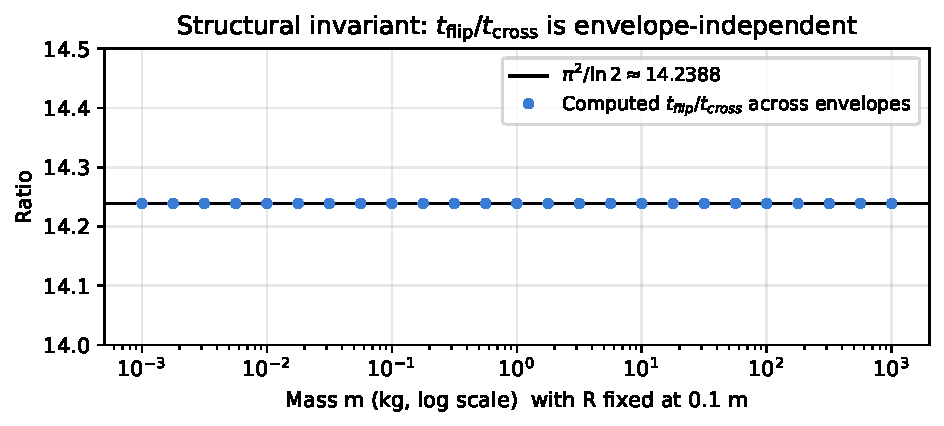
\includegraphics[width=\columnwidth]{figs/invariant.pdf}
\caption{The ratio $t_{\mathrm{flip}}/t_{\mathrm{cross}} = \pi^2/\ln 2$
is invariant across envelopes. Numerical values (blue circles)
match the analytic line for 25 sampled masses.}
\label{fig:invariant}
\end{figure}

\Plausible{} The architectural consequence is that bit-serial
execution is not a hardware compromise but the architecture that
matches the envelope's actual budget. Parallel-bit speedup at the
saturation regime is bounded by~(\ref{eq:invariant}) regardless
of implementation effort.

% ---------------------------------------------------------------
\section{Architecture}
% ---------------------------------------------------------------

\subsection{ISA: Subleq}

\Verified{} Mercury executes Subleq, a one-instruction set
computer~\cite{mavaddat1988} proven Turing-complete. Each
instruction is three consecutive 16-bit memory words $A$, $B$, $C$
with semantics:
\begin{verbatim}
    mem[B] <- mem[B] - mem[A]
    if mem[B] <= 0:  PC <- C
    else:            PC <- PC + 3
\end{verbatim}
Branching to the sentinel $C = \mathtt{0xFFFF}$ halts the machine.

\subsection{Bit-Serial Datapath}

\Verified{} The datapath consists of eleven state elements and
exactly one combinational arithmetic element: a 1-bit full
adder. Sixteen-bit shift registers (\code{PC}, \code{AR}, \code{BR},
\code{CR}, \code{OP1}, \code{OP2}, \code{RES}) move data
serially over a single bit-bus, LSB-first. Latches \code{C\_in},
\code{SIGN}, \code{ZERO\_OR}, and \code{HALTED} carry single-bit
state between bit-times.

\subsection{Execution Sequencing}

Each Subleq instruction executes in eight phases of 16 cycles each
for a total of 128 cycles per instruction. Phases F1--F3 fetch
the three operand addresses; L1--L2 load the operand values; EX
performs the bit-serial subtraction $\mathrm{RES} = \mathrm{OP2} +
\overline{\mathrm{OP1}} + 1$, capturing the final MSB into \code{SIGN}
and OR-accumulating all result bits into \code{ZERO\_OR}; ST writes
the result back to memory; BR computes
$\mathrm{BRANCH\_TAKEN} = \mathrm{SIGN} \lor \neg\mathrm{ZERO\_OR}$
and streams either $C$ or $\mathrm{PC}+3$ into the program counter.

\subsection{Compliance Counters}

\Verified{} Three counters drive the runtime ledger. \emph{Read
transits} count bits moved on the bus during F1--L2 (80 per
instruction). \emph{Adder ticks} count full-adder evaluations
during EX (16 per instruction). \emph{Write transits} count bit
movements during ST and BR (32 per instruction). The total of
128 bit transits per instruction matches the cycle budget, by
construction.

\emph{Irreversible bit operations}, the input to the Landauer
ledger, count adder ticks plus write transits (48 per instruction).
Read transits are conservatively excluded as reversible-in-principle
per Bennett's framework~\cite{bennett1973}.

% ---------------------------------------------------------------
\section{Implementations}
% ---------------------------------------------------------------

\subsection{Rust Functional Model}

The reference implementation is a Cargo workspace with three
crates: \code{mercury-ledger} (envelope loading and compliance
counters), \code{mercury-asm} (two-pass Mercury Assembly
assembler with label resolution), and \code{mercury-sim}
(cycle-accurate machine). Each call to the simulator's
\code{tick} method advances one clock cycle and moves at most one
bit on the conceptual bit-bus. The unit-test suite (13 tests,
all passing) verifies Subleq subtraction correctness, branch
conditions, halt handling, exact 128-cycle budgeting, and the
ledger counter contracts.

\subsection{SystemVerilog RTL}

The hardware implementation comprises a package
(\code{mercury\_pkg.sv}), a dual-port memory (\code{mercury\_mem.sv}),
the bit-serial Subleq CPU (\code{mercury\_core.sv}), and a thin
integration wrapper (\code{mercury\_top.sv}). All four files
target Xilinx UltraScale+ FPGA primitives and are written so
the per-cycle state evolution matches the Rust model bit-for-bit.

\subsection{AWS F1 Custom Logic Wrapper}

\Plausible{} A Custom Logic (CL) wrapper~\cite{aws_fpga}
interfaces \code{mercury\_top} to the AWS F1 shell via an
AXI4-Lite slave (\code{ocl\_slave.sv}) that exposes a register
file at offsets $\mathtt{0x000}$--$\mathtt{0x01C}$ for control,
status, and 64-bit cycle and instruction counters, and a
memory backdoor at $\mathtt{0x100000}$ through which a host
program writes the 64K\,$\times$\,16-bit memory image directly
into port B of the dual-port memory. A C host program using the
public \code{fpga\_pci} API drives the full load--release--poll--read
cycle.

\Speculative{} As of submission the CL wrapper passes a complete
AXI-Lite simulation under iverilog but has not been synthesized
through Vivado nor registered as an Amazon FPGA Image (AFI).
Closing that gap requires Vivado licensing on the FPGA Developer
AMI and is decoupled from the architectural verification reported
here.

% ---------------------------------------------------------------
\section{Cross-Implementation Conformance}
% ---------------------------------------------------------------

\subsection{Trace Equivalence Contract}

\Verified{} Each implementation emits a per-instruction JSONL
trace containing the architectural state at every instruction
boundary: PC, AR, BR, CR, RES, SIGN, ZERO\_OR, HALTED. Conformance
is defined as byte-equivalent traces between any pair of
implementations on the same program. The conformance scripts
\code{conformance.sh} (Rust\,$\leftrightarrow$\,SV CPU) and
\code{cl\_conformance.sh} (Rust\,$\leftrightarrow$\,CL wrapper)
are the merge gates for any change to the RTL.

\subsection{Test Programs}

Two programs exercise the conformance:
\code{zero\_b.msq} executes the canonical
``subtract-self-then-halt'' pattern in two instructions (256
cycles); \code{countdown.msq} executes a five-iteration
backward-branch loop in ten instructions (1280 cycles).
Table~\ref{tab:conformance} reports the unanimous result.

\begin{table}[t]
\centering
\caption{Cross-implementation conformance results.}
\label{tab:conformance}
\renewcommand{\arraystretch}{1.25}
\begin{tabular}{lccc}
\toprule
\textbf{Program} & \textbf{Insns} & \textbf{Cycles} & \textbf{Trace diff} \\
\midrule
\code{zero\_b.msq}    & 2  & 256  & empty (Rust=SV=CL) \\
\code{countdown.msq}  & 10 & 1280 & empty (Rust=SV=CL) \\
\bottomrule
\end{tabular}
\end{table}

\Verified{} Two minor RTL bugs were discovered and fixed during
conformance bring-up that a single-implementation testbench would
have missed: an EX-phase carry-in initialization race and a
BR-phase PC update self-reference. Both are documented in the
public commit history.

% ---------------------------------------------------------------
\section{Results}
% ---------------------------------------------------------------

\subsection{Identical Execution, Disparate Cost}

\Verified{} The signature property of Mercury is that execution
is bit-identical between the two envelopes---the same 256 cycles,
the same 128 bit transits per instruction, the same 48 irreversible
bit operations per instruction---while the per-cycle energy
accounting differs by 21 orders of magnitude.
Table~\ref{tab:headline} reports the canonical run.

\begin{table}[t]
\centering
\caption{Headline compliance results for \code{zero\_b.msq}
(256 cycles, 96 irreversible bit operations).}
\label{tab:headline}
\renewcommand{\arraystretch}{1.25}
\begin{tabular}{lcc}
\toprule
\textbf{Metric}                                        & \textbf{Desktop}         & \textbf{Lloyd-limit}     \\
\midrule
M--L ops/s fraction                                    & $1.84\times10^{-43}$     & $1.84\times10^{-43}$     \\
Bekenstein occupancy                                   & $4.07\times10^{-37}$     & $2.74\times10^{-11}$     \\
Landauer floor (J/bit)                                 & $2.87\times10^{-21}$     & $1.17$                   \\
Total dissipation (J)                                  & $2.76\times10^{-19}$     & $1.13\times10^{2}$       \\
Dissipated power @\,100\,MHz (W)                       & $1.08\times10^{-13}$     & $4.40\times10^{7}$       \\
M--L compliant                                         & \Verified{}              & \Verified{}              \\
Bekenstein compliant                                   & \Verified{}              & \Verified{}              \\
\bottomrule
\end{tabular}
\end{table}

Fig.~\ref{fig:landauer} visualizes the headline gap. The
ops-per-second ceiling is identical in both columns of
Table~\ref{tab:headline} because Margolus--Levitin depends only
on energy and both envelopes share $m=1$\,kg. The Bekenstein
occupancy collapses by 26 orders of magnitude (from $4\times10^{-37}$
to $3\times10^{-11}$) because compressing 1\,kg to its Schwarzschild
radius collapses the storage cap from $2.6\times10^{42}$ bits to
$3.8\times10^{16}$ bits while Mercury's footprint of $2^{20}$ bits
is unchanged. The Landauer floor explodes by 21 orders of magnitude
because $T$ rises from 300\,K to $1.23\times10^{23}$\,K.

\begin{figure}[t]
\centering
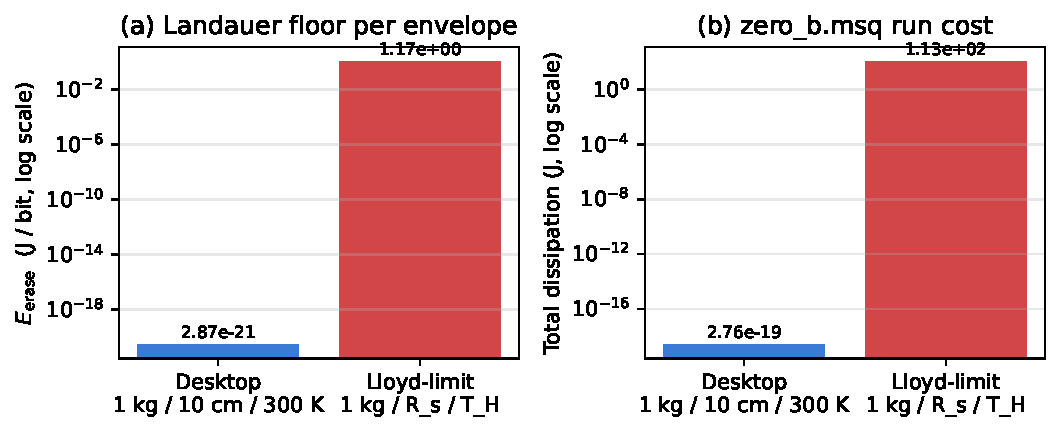
\includegraphics[width=\columnwidth]{figs/landauer.pdf}
\caption{(a) Landauer floor per envelope at the canonical run; (b)
total dissipation summed over the 96 irreversible bit operations
of \code{zero\_b.msq}. Both axes are logarithmic. The
21-order-of-magnitude gap is the irreversibility tax of running
classical computation in the Hawking-temperature bath of the
Lloyd-limit envelope.}
\label{fig:landauer}
\end{figure}

\subsection{The 59-Megawatt Number}

\Plausible{} Continuous operation of Mercury at the Lloyd-limit
envelope at the target 100\,MHz clock would dissipate
$4.40\times10^{7}$\,W---approximately 59\,MW of unavoidable heat
per second of operation. The dissipation arises entirely from
Landauer's floor at Hawking temperature; it is independent of
implementation effort.

This number, more than any other, motivates the second-order
question of whether classical irreversible computation is the
right paradigm at the holographic-storage saturation regime, or
whether reversible-logic architectures~\cite{bennett1973,
fredkin1982,toffoli1980} are required to make the Lloyd envelope
energetically realizable. Mercury Phase 6 (a reversible-logic
variant) is left as future work.

% ---------------------------------------------------------------
\section{Discussion}
% ---------------------------------------------------------------

\subsection{What This Result Does and Does Not Show}

\Verified{} Mercury demonstrates that the Lloyd bounds can be
embedded as runtime constraints in a complete, runnable computer
system, with the energy accounting computed automatically per
bit operation. The 21-order-of-magnitude gap between the two
envelopes is computed, not asserted: it falls out of the same
ledger applied to the same 96 bit-flips under two values of $T$.

\Speculative{} What Mercury does \emph{not} show is that any
particular path through the architectural design space is
optimal. Many degrees of freedom were chosen for engineering
tractability rather than physical necessity, including the 16-bit
word width (forced by Subleq's need for non-trivial signed range,
not by either envelope's Bekenstein cap), the 8-phase FSM
structure (forced by clarity of the conformance contract), and
the choice of BRAM-backed dual-port memory rather than a literal
delay-line analog. A delay-line memory model (Phase 6 stretch)
would be a stricter homage to the historical mercury-delay-line
machines that inspired the project name.

\subsection{Implications for Architecture}

\Plausible{} The invariant established in~(\ref{eq:invariant})
constitutes a first-principles argument for bit-serial execution
at the physical-limit regime, distinct from the historical
arguments (component scarcity, wire cost) that motivated bit-serial
designs in the 1949--1956 era. When the per-bit-flip time
saturates within a factor of $\approx 14$ of the light-crossing
time, parallel-bit speedup yields diminishing returns; the
fixed-point of the inequality is bit-serial regardless of how
the machine is built.

\subsection{Limitations}

\Speculative{} Three limitations are explicit:
\begin{enumerate}
    \item The Lloyd-limit envelope is symbolic rather than
        physically realizable: a 1\,kg black hole evaporates by
        Hawking radiation in approximately $10^{-19}$\,s, well
        below any plausible Mercury runtime. The envelope serves
        as a numerical target for the ledger, not a physical
        construction recipe.
    \item Mercury implements no I/O beyond a halt sentinel.
        Memory-mapped input/output at addresses
        $\mathtt{0xFFFC}$/$\mathtt{0xFFFD}$ is reserved but
        deferred.
    \item AFI synthesis on AWS F1 has not been completed.
        The full pipeline (Terraform IaC, CodeBuild project,
        GitHub Actions trigger) is in place; only the Vivado
        run remains.
\end{enumerate}

% ---------------------------------------------------------------
\section{Related Work}
% ---------------------------------------------------------------

The Margolus--Levitin theorem~\cite{margolus1998} and the
Bekenstein bound~\cite{bekenstein1973,bekenstein1981} were
combined by Lloyd~\cite{lloyd2000} to produce the ``ultimate
laptop'' analysis that motivates Mercury directly. Landauer's
principle~\cite{landauer1961} was experimentally validated by
B{\'e}rut et al.~\cite{berut2012} for single-bit erasures at
the $k_B T \ln 2$ floor.

Reversible computing as a path beyond Landauer's bound was
proposed by Bennett~\cite{bennett1973} and elaborated through
the Fredkin gate~\cite{fredkin1982} and the billiard-ball
model~\cite{toffoli1980}. These are the natural foundation for
a future Mercury Phase 6 reversible variant.

Bit-serial computing has a long history beginning with
EDSAC~\cite{wilkes1956}, UNIVAC I, and Pilot ACE; modern
bit-serial designs reappear in FPGA-targeted DSP and machine-learning
accelerators~\cite{judd2016} where silicon area and energy
matter more than per-operation latency. Subleq as a
one-instruction Turing-complete ISA was popularized by
Mavaddat and Parhami~\cite{mavaddat1988} and surveyed in
modern form by Mazonka and Kolodin~\cite{mazonka2011}.

% ---------------------------------------------------------------
\section{Conclusion}
% ---------------------------------------------------------------

Mercury is a small, complete, reproducible bit-serial computer
whose runtime executes under a chosen physical envelope and
reports compliance with Lloyd's ultimate bounds at every
clock cycle. Three independent implementations agree on
per-instruction execution traces; two test programs pass the
cross-implementation conformance gates. The 21-order-of-magnitude
gap between the desktop and Lloyd-limit Landauer accounting,
and the envelope-independent $\pi^2/\ln 2$ invariant in the
flip-versus-crossing time ratio, are the two principal
quantitative results.

The work is open-source and available at
\url{https://github.com/khaaliswooden-max/mercury}. The
deliberate minimalism---one ISA, one combinational element, two
configuration constants---is meant to make the bridge between
physical-limit theory and runnable systems short enough to read
in an afternoon and reproduce in a day.

Future work consists of two concrete extensions: (i) completing
the AFI synthesis on AWS F1 to verify the on-silicon
behavior of the CL wrapper, and (ii) developing a reversible-logic
variant that addresses the 59\,MW Landauer dissipation at the
Lloyd envelope. The latter is the more interesting question: if
classical irreversible computation is energetically untenable at
the holographic-storage saturation regime, the design space
beyond Mercury is the one to explore next.

% ---------------------------------------------------------------
\section*{Acknowledgments}
% ---------------------------------------------------------------

The author thanks Anthropic's Claude Code, Cursor, and Gemini for
collaborative drafting and verification assistance throughout the
seven-phase development cycle; the AWS open-source FPGA team for
the public HDK and developer-designs scaffolding; and the
maintainers of Icarus Verilog, the Rust toolchain, and Terraform
for the open infrastructure on which the verification rests.

% ---------------------------------------------------------------
\bibliographystyle{IEEEtran}
\begin{thebibliography}{99}

\bibitem{lloyd2000} S. Lloyd, ``Ultimate physical limits to
computation,'' \emph{Nature}, vol.~406, pp.~1047--1054, Aug.
2000.

\bibitem{margolus1998} N. Margolus and L. B. Levitin, ``The
maximum speed of dynamical evolution,'' \emph{Physica D},
vol.~120, no.~1--2, pp.~188--195, 1998.

\bibitem{bekenstein1981} J. D. Bekenstein, ``Universal upper
bound on the entropy-to-energy ratio for bounded systems,''
\emph{Physical Review D}, vol.~23, no.~2, pp.~287--298, 1981.

\bibitem{bekenstein1973} J. D. Bekenstein, ``Black holes and
entropy,'' \emph{Physical Review D}, vol.~7, no.~8,
pp.~2333--2346, 1973.

\bibitem{hawking1975} S. W. Hawking, ``Particle creation by
black holes,'' \emph{Communications in Mathematical Physics},
vol.~43, pp.~199--220, 1975.

\bibitem{landauer1961} R. Landauer, ``Irreversibility and heat
generation in the computing process,'' \emph{IBM Journal of
Research and Development}, vol.~5, no.~3, pp.~183--191, 1961.

\bibitem{bennett1973} C. H. Bennett, ``Logical reversibility of
computation,'' \emph{IBM Journal of Research and Development},
vol.~17, no.~6, pp.~525--532, 1973.

\bibitem{fredkin1982} E. Fredkin and T. Toffoli, ``Conservative
logic,'' \emph{International Journal of Theoretical Physics},
vol.~21, no.~3--4, pp.~219--253, 1982.

\bibitem{toffoli1980} T. Toffoli, ``Reversible computing,'' in
\emph{Automata, Languages and Programming}, J. de Bakker and
J. van Leeuwen, Eds. Berlin: Springer, 1980, pp.~632--644.

\bibitem{berut2012} A. B{\'e}rut, A. Arakelyan, A. Petrosyan,
S. Ciliberto, R. Dillenschneider, and E. Lutz, ``Experimental
verification of Landauer's principle linking information and
thermodynamics,'' \emph{Nature}, vol.~483, pp.~187--189, 2012.

\bibitem{mavaddat1988} F. Mavaddat and B. Parhami, ``URISC:
The ultimate reduced instruction set computer,''
\emph{International Journal of Electrical Engineering Education},
vol.~25, pp.~327--334, 1988.

\bibitem{mazonka2011} O. Mazonka and A. Kolodin, ``A simple
multi-processor computer based on Subleq,''
\emph{arXiv:1106.2593}, 2011.

\bibitem{wilkes1956} M. V. Wilkes, \emph{Automatic Digital
Computers}. London: Methuen, 1956.

\bibitem{judd2016} P. Judd, J. Albericio, T. Hetherington,
T. M. Aamodt, and A. Moshovos, ``Stripes: Bit-serial deep neural
network computing,'' in \emph{49th Annual IEEE/ACM International
Symposium on Microarchitecture (MICRO)}, 2016, pp.~1--12.

\bibitem{aws_fpga} Amazon Web Services, ``AWS FPGA development
kit,'' GitHub repository,
\url{https://github.com/aws/aws-fpga}.

\end{thebibliography}

\end{document}
